\section{DevOps}\label{devops}
The project utilizes a series of services to facilitate the production cycle, starting from version control combined with automation that finally then to simplified releases.

GitHub was chosen as the primary hub for the code base. In particular the "GitHub organizations" feature of such service allows creating organizations where people can cooperate and, most importantly, groups together repositories belonging to that specific organization, separating them from personal accounts.

\begin{figure}[!ht]
    \centering
    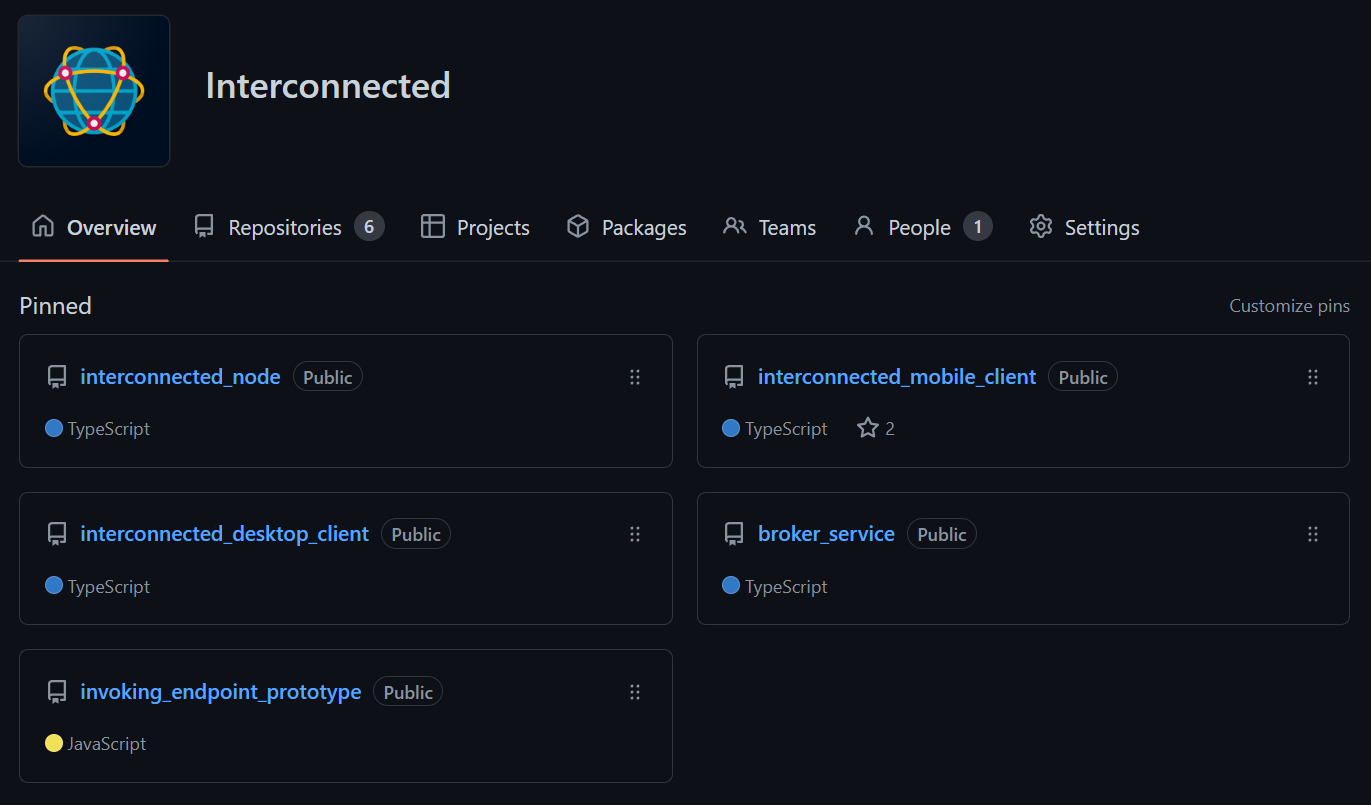
\includegraphics[width=\linewidth]{document/chapters/chapter_7/images/interconnected_organization.png}
    \caption{Interconnected - GitHub Organization}
    \label{fig:interconnected_organization}
\end{figure}

Furthermore, through the definition of specific GitHub actions, a lot of repetitive tasks can be automated; in this project case, actions collaborate with external services in order to obtain CD (Continuous Delivery) automation.

The first external service used is NPM; when a new release of the Interconnected Node is created, a GitHub action uses the repository's code base in order to publish the module on NPM (\textit{figure \ref{fig:interconnected_npm}}), making it available for the Mobile and Desktop Contributing Endpoints.

\begin{figure}[!ht]
    \centering
    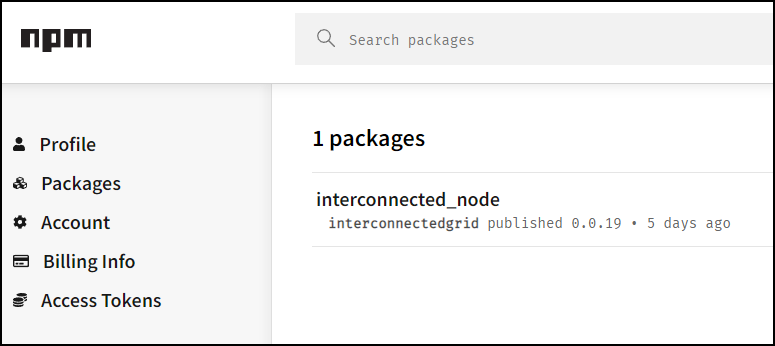
\includegraphics[scale=0.45]{document/chapters/chapter_7/images/interconnected_npm.png}
    \caption{Interconnected - NPM}
    \label{fig:interconnected_npm}
\end{figure}

The Broker Service and the Interconnected Desktop Client both utilize Docker for the execution on target machines; such Docker images are automatically created and published on Docker Hub whenever a new release is created in the respective repositories. Thanks to this, a machine that wants to run a container with that specific image will not need to access the code base and run, compile and run the Node.js environment but will only need a working installation of the Docker client; knowing the image name, this will automatically be downloaded from Docker Hub to the target machine (\textit{figure \ref{fig:interconnected_desktop}}). 

\begin{figure}[!ht]
    \centering
    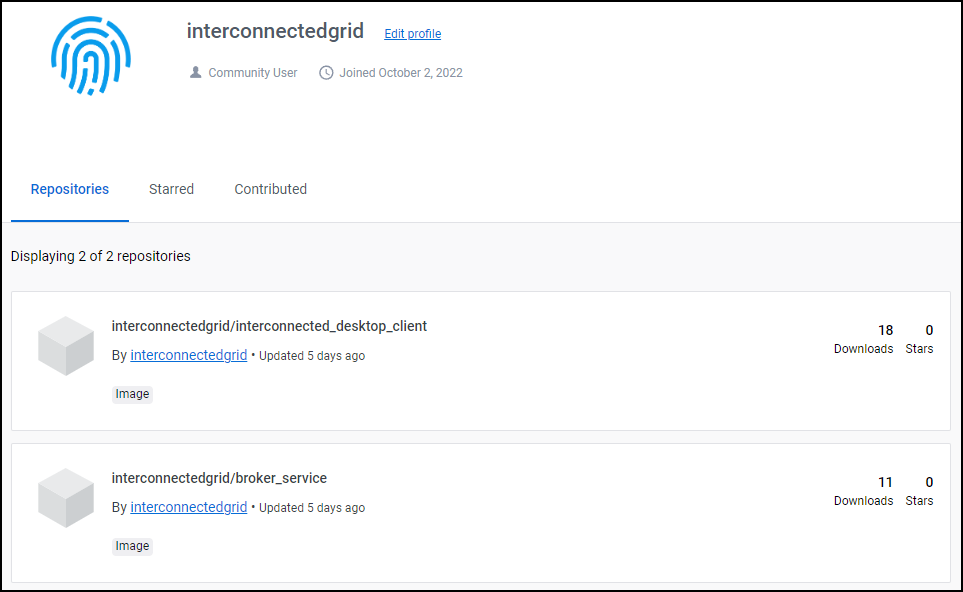
\includegraphics[width=\linewidth]{document/chapters/chapter_7/images/interconnected_dockerhub.png}
    \caption{Interconnected - Docker Hub}
    \label{fig:interconnected_dockerhub}
\end{figure}

In particular, when it comes to the execution of the Broker Service's image on a container, Amazon ECS offers a simple hosting platform that is able to pull images from Docker Hub by simply defining a task and running it. This way, every time the Broker Service is started, Amazon ECS' defined task will retrieve the latest published image and will run it on a dedicated container (\textit{figure \ref{fig:interconnected_ecs}}).

\begin{figure}[!ht]
    \centering
    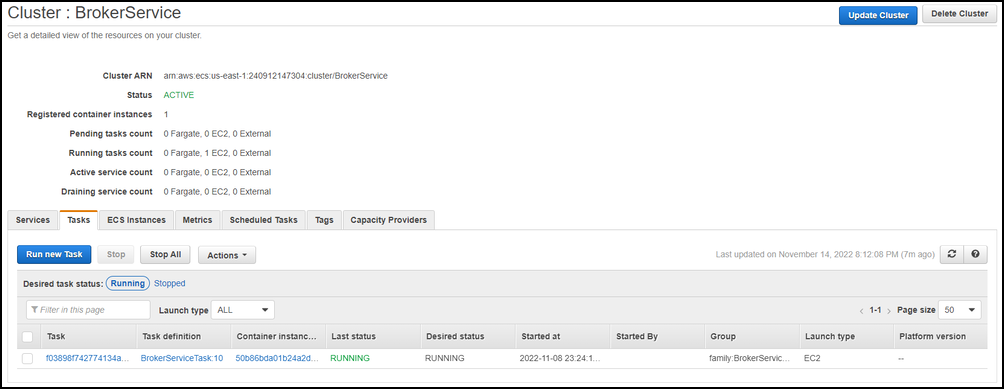
\includegraphics[width=\linewidth]{document/chapters/chapter_7/images/interconnected_ecs.png}
    \caption{Interconnected - Amazon ECS}
    \label{fig:interconnected_ecs}
\end{figure}

Finally, despite being run on an emulator during development, the Interconnected Mobile Client needs to be delivered in production; each time a new release is created on it's GitHub repository, an action will build an APK and publish it as an attached file to said release. This way, a ready-to-use installer is automatically made available for installation on real Android devices.

\begin{figure}[!ht]
    \centering
    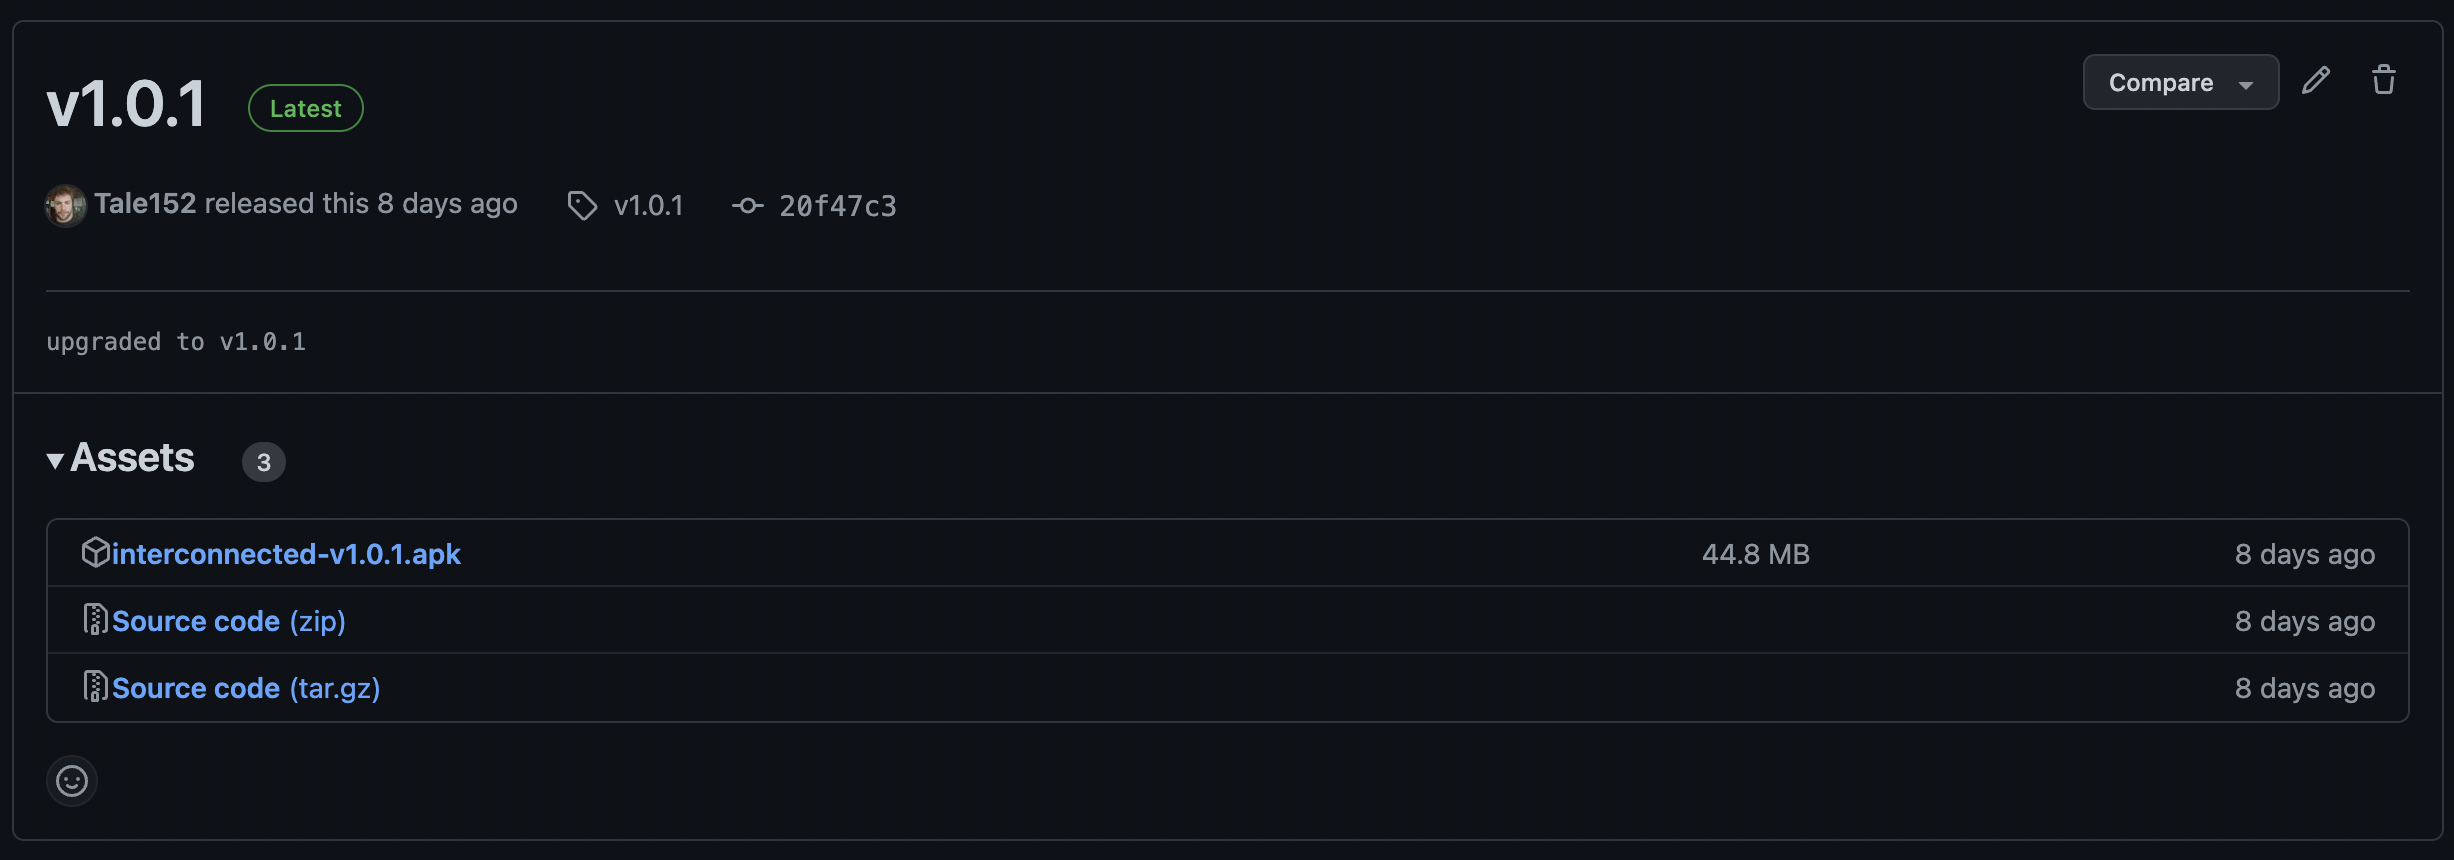
\includegraphics[scale=0.35]{document/chapters/chapter_7/images/github_actions_apk.png}
    \caption{Android APK automated release}
    \label{fig:github_actions_apk}
\end{figure}